\documentclass[12pt]{article}
\usepackage[utf8]{inputenc}
\usepackage[margin=1in]{geometry}
\usepackage[spanish]{babel}\decimalpoint
\usepackage{setspace}\onehalfspacing
\usepackage{parskip} % Espacio entre parrafos.
\usepackage{graphicx} % Para usar comando \includegraphics[]{}
\usepackage{amssymb} % Para usar el simbolo del conj. de los Reales.
\usepackage{amsmath} % Para usar columnas vectoriales.
\usepackage{multirow} % Para unir multiples filas en una tabla.
\usepackage{hyperref} % Siempre debe ser el ultimo paquete.


\setcounter{tocdepth}{2} % Que no incluya subsubsections en la tabla de contenidos (toc).

%================================

\title{Clase 2. Los Determinantes y el Producto Cruz.}
\author{MIT 18.02: Multivariable Calculus.}
\date{}


\begin{document}

\maketitle

\begin{abstract}
\noindent Para comenzar, haremos una revisión breve de otra aplicación del producto punto al calcular el componente de un vector a lo largo (o en dirección) de otro. Posteriormente, nos concentraremos en estudiar los determinantes y el producto cruz.
\end{abstract}


\section{Componente de un vector a lo largo de otro.}

El producto punto, además de ser útil para evaluar si dos vectores son ortogonales o para conocer la magnitud de uno de ellos, también es de ayuda para obtener el componente de un vector en dirección de (o a lo largo de) otro.

En la clase anterior estudiamos que es posible representar a un vector como la combinación lineal entre sus componentes y vectores unitarios estándar. Por ejemplo:
\[
  \mathbf{a} = a_{1} \hat{\mathbf{i}} + a_{2} \hat{\mathbf{j}} = \langle a_{1}, \ a_{2} \rangle
\]
donde $a_{1} = |x_{2} - x_{1}|$, $a_{2} = |y_{2} - y_{1}|$, $\hat{\mathbf{i}} = \langle 1, \ 0 \rangle$ y $\hat{\mathbf{j}} = \langle 0, \ 1 \rangle$. A continuación lo vemos de forma gráfica:

\begin{figure}[hbt!]
\centering
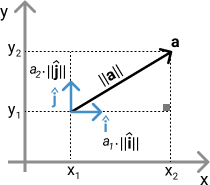
\includegraphics[scale=0.7]{img/vect-along-other-1.jpg}
\end{figure}

En ese sentido, podemos decir que $a_{1}$ es el componente del vector $\mathbf{a}$ que va en la dirección de $\hat{\mathbf{i}}$. Lo mismo se aplica para $a_{2}$, pero con respecto a $\hat{\mathbf{j}}$.

Ahora, si bien en este caso es fácil conocer a los componentes\footnote{$a_{1} \cdot ||\hat{\mathbf{i}}|| = a_{1}$ porque $||\hat{\mathbf{i}}|| = 1$. Lo mismo con $a_{2}$.} de $\mathbf{a}$, busquemos una forma de calcularlos.

Veamos en el componente $a_{1}$. Como pudimos observar en el gráfico de arriba, entre $\mathbf{a}$ y $\hat{\mathbf{i}}$ se forma el siguiente triángulo rectángulo:

\begin{figure}[hbt!]
\centering
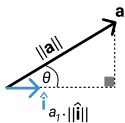
\includegraphics[scale=0.7]{img/vect-along-other-2.jpg}
\end{figure}

Nuestro interés es conocer a $a_{1} \cdot ||\hat{\mathbf{i}}||$. Si conocemos el $\angle \theta$ y al tener el triángulo rectángulo, podemos obtener este lado a partir del $\cos(\theta)$.
\begin{align*}
  \cos(\theta) &= \frac{a_{1} \cdot ||\hat{\mathbf{i}}||}{||\mathbf{a}||} \\
  ||\mathbf{a}|| \cdot \cos(\theta) &= a_{1} \cdot ||\hat{\mathbf{i}}||
\end{align*}
Esta fórmula es útil si conocemos a $\angle \theta$. Si no es el caso, recordemos que es el ángulo entre dos vectores: $\mathbf{a}$ y $\hat{\mathbf{i}}$. Por lo tanto, podemos usar la fórmula geométrica del producto punto y despejar el $\cos(\theta)$ en ella.
\begin{align*}
  \mathbf{a} \cdot \hat{\mathbf{i}} = ||\mathbf{a}|| \cdot ||\hat{\mathbf{i}}|| \cdot \cos(\theta) \\
  \frac{\mathbf{a} \cdot \hat{\mathbf{i}}}{||\mathbf{a}|| \cdot ||\hat{\mathbf{i}}||} &= \cos(\theta) 
\end{align*}
Luego, reemplacemos el $\cos(\theta)$ en la ecuación de $a_{1} \cdot ||\hat{\mathbf{i}}||$.
\begin{align*}
||\mathbf{a}|| \cdot \cos(\theta) &= a_{1} \cdot ||\hat{\mathbf{i}}|| \\
||\mathbf{a}|| \cdot \left(\frac{\mathbf{a} \cdot \hat{\mathbf{i}}}{||\mathbf{a}|| \cdot ||\hat{\mathbf{i}}||}\right) &= a_{1} \cdot ||\hat{\mathbf{i}}|| \\
\frac{\mathbf{a} \cdot \hat{\mathbf{i}}}{||\hat{\mathbf{i}}||} &= a_{1} \cdot ||\hat{\mathbf{i}}|| 
\end{align*}
Esta fórmula la podemos generalizar para cualquier par de vectores.

Si tenemos dos vectores $\mathbf{a}$ y $\mathbf{b}$ no nulos, podemos conocer el componente $c$ del primero a lo largo del segundo por medio de estas dos fórmulas:
\[
  c = ||\mathbf{a}|| \cdot \cos(\theta) \qquad \text{o} \qquad
  c = \frac{\mathbf{a} \cdot \mathbf{b}}{||\mathbf{b}||} = \mathbf{a} \cdot \left(\frac{\mathbf{b}}{||\mathbf{b}||}\right)
\]
donde $c$ es un \textbf{escalar}.

El componente de un vector sobre otro también se conoce como \textbf{proyección escalar} de $\mathbf{a}$ sobre $\mathbf{b}$, porque lo que estamos haciendo es proyectar al primero a lo largo del segundo.

\begin{figure}[hbt!]
\centering
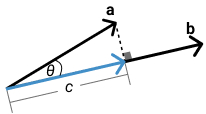
\includegraphics[scale=0.7]{img/scalar-proj-1.jpg}
\end{figure}

Como vemos, la proyección de $\mathbf{a}$ sobre $\mathbf{b}$ es un vector y su magnitud es $c$, el componente del primero a lo largo o en dirección del segundo.

Por otra parte, si $0 < \theta < 90^{\circ}$, $c > 0$. En cambio, si $90^{\circ} < \theta < 180^{\circ}$, $c < 0$.

\begin{figure}[hbt!]
\centering
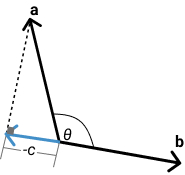
\includegraphics[scale=0.6]{img/scalar-proj-2.jpg}
\end{figure}

En Álgebra Lineal se profundiza más sobre proyecciones.



\section{Determinantes.}

En esta ocasión no profundizaremos en la definición de los \textbf{Determinantes}, pero sí es bueno resaltar en que es un \textbf{número} (o un escalar) muy utilizado en áreas de la matemática (álgebra lineal, por ejemplo) o la física. Por ahora nos centraremos en su interpretación geométrica y su fórmula la usaremos simbólicamente en la siguiente sección.

\subsection{Determinantes en el Plano.}

Si tenemos dos vectores no nulos en dos dimensiones $\mathbf{a} = \langle a_{1}, \ a_{2} \rangle$ y $\mathbf{b} = \langle b_{1}, \ b_{2} \rangle$, es posible calcular un número con sus componentes llamado \textbf{determinante}:
\[
\det(\mathbf{a}, \ \mathbf{b}) =
  \begin{vmatrix}
  a_{1} & a_{2} \\
  b_{1} & b_{2}
  \end{vmatrix} =
  a_{1}b_{2} - a_{2}b_{1}
\]
A nivel geométrico, el determinante de $\mathbf{a}$ y $\mathbf{b}$ de dos dimensiones coincide con ser el valor absoluto del \textbf{área del paralelógramo} que es posible formar entre los dos vectores.

\begin{figure}[hbt!]
\centering
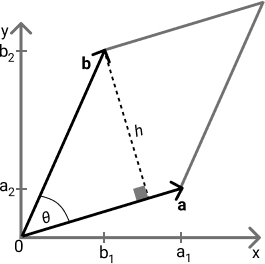
\includegraphics[scale=0.6]{img/det-area-parallelog-1.jpg}
\end{figure}

Formalmente, el área de un paralelógramo, que denotaremos como $A_{P}$, se calcula como:
\[
  A_{P} = \text{base} \cdot \text{altura}
\]
En este caso, la base es $||\mathbf{a}||$ y la altura podemos obtenerla a partir del $\sin(\theta)$:
\begin{align*}
  \sin(\theta) &= \frac{h}{||\mathbf{b}||} \\
  ||\mathbf{b}|| \cdot \sin(\theta) &= h
\end{align*}
Por lo tanto:
\[
  A_{P} = ||\mathbf{a}|| \cdot ||\mathbf{b}|| \cdot \sin(\theta)
\]
La fórmula de arriba es útil si conocemos al $\angle \theta$, pero nuestra idea es conocer el $A_{P}$ a partir de las componentes de $\mathbf{a}$ y $\mathbf{b}$. Podríamos trabajar con el producto punto entre ambos, pero necesitamos al $\cos(\cdot)$ y no al $\sin(\cdot)$. Una estrategia que podemos tomar, es rotar al vector $\mathbf{a}$ en $\pi/2$ radianes (i.e, $90^{\circ}$), obteniendo a $\mathbf{a}' = \langle -a_{2}, \ a_{1} \rangle$.

\newpage

\begin{figure}[hbt!]
\centering
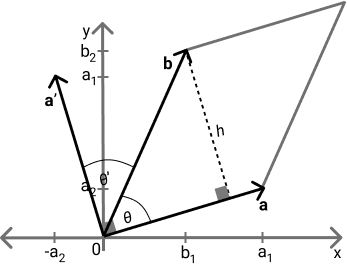
\includegraphics[scale=0.6]{img/det-area-parallelog-2.jpg}
\end{figure}

Veamos que $\theta '$ es complementario a $\theta$, donde $\theta + \theta ' = \pi/2$, implicando que:
\[
  \theta ' = \frac{\pi}{2} - \theta
\]
Debido a que $\theta$ y $\theta '$ son complementarios, podemos asumir que $\sin(\theta) = \cos(\theta ')$. Para demostrarlo, usamos la fórmula de sustracción del coseno\footnote{Stewart, et al (2017). \textit{Precálculo. Matemáticas para el Cálculo}. Pp. 500 y 502.}:
\begin{align*}
\sin(\theta) &= \cos(\theta ') \\
\sin(\theta) &= \cos\left(\frac{\pi}{2} - \theta\right) \\
\sin(\theta) &= \cos\left(\frac{\pi}{2}\right) \cdot \cos(\theta) + \sin\left(\frac{\pi}{2}\right) \cdot \sin(\theta) \\
\sin(\theta) &= \sin(\theta) \ \text{(Q.E.D)}
\end{align*}
Observemos, también, que $||\mathbf{a}'|| = ||\mathbf{a}||$. Por lo tanto, podemos sostener sin alterar nada que:
\[
  A_{P} = ||\mathbf{a}'|| \cdot ||\mathbf{b}|| \cdot \cos(\theta ')
        = \mathbf{a}' \cdot \mathbf{b}
        = -a_{2}b_{1} + a_{1}b_{2}
        = a_{1}b_{2} - a_{2}b_{1}
        = \begin{vmatrix}
          a_{1} &  a_{2} \\
          b_{1} &  b_{2}
          \end{vmatrix}
        = \det(\mathbf{a}, \ \mathbf{b})
\]
Ahora bien, \textbf{el determinante puede ser positivo o negativo}.
\[
\det(\mathbf{a}, \ \mathbf{b}) =
\pm
\begin{vmatrix}
a_{1} &  a_{2} \\
b_{1} &  b_{2}
\end{vmatrix}
\]
Por lo tanto, el área del paralelógramo $A_{p}$ es igual al \textbf{valor absoluto} del $\det(\mathbf{a}, \ \mathbf{b})$.
\[
  A_{P} = |\det(\mathbf{a}, \ \mathbf{b})|
\]

De modo similar, podemos decir que:
\[
  \det(\mathbf{a}, \ \mathbf{b}) = \pm A_{P}
\]

\subsection{Determinantes en el Espacio.}

Si tenemos tres vectores en tres dimensiones $\mathbf{a} = \langle a_{1}, \ a_{2}, \ a_{3} \rangle$, $\mathbf{b} = \langle b_{1}, \ b_{2}, \ b_{3} \rangle$ y $\mathbf{c} = \langle c_{1}, \ c_{2}, \ c_{3} \rangle$, su determinante $\det(\mathbf{a}, \ \mathbf{b}, \ \mathbf{c})$ se calcula como:
\[
\det(\mathbf{a}, \ \mathbf{b}, \ \mathbf{c}) =
\begin{vmatrix}
a_{1} & a_{2} & a_{3} \\
b_{1} & b_{2} & b_{3} \\
c_{1} & c_{2} & c_{3} 
\end{vmatrix} =
a_{1}
\cdot
\begin{vmatrix}
b_{2} & b_{3} \\
c_{2} & c_{3}
\end{vmatrix}
-
a_{2}
\cdot
\begin{vmatrix}
b_{1} & b_{3} \\
c_{1} & c_{3}
\end{vmatrix}
+
a_{3}
\cdot
\begin{vmatrix}
b_{1} & b_{2} \\
c_{1} & c_{2}
\end{vmatrix}
\]
El proceso aplicado a esta determinante se conoce como \textbf{expansión por la primera fila}. Es un concepto que se entiende mejor al trabajar con matrices, por lo tanto no profundizaremos en ello.

Lo principal a destacar, es que el determinante de tres vectores en el espacio coincide con ser igual al \textbf{volumen de un paralelepipedo} (i.e, el sólido del paralelógramo) que se puede formar con ellos.

\begin{figure}[hbt!]
\centering
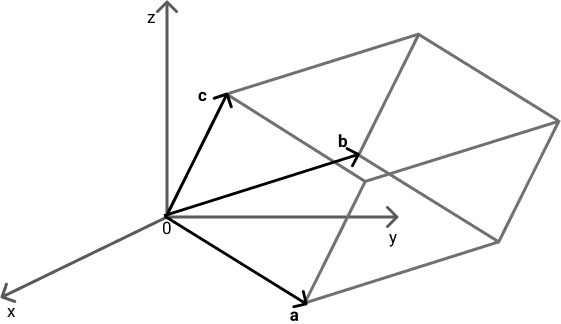
\includegraphics[scale=0.4]{img/det-vol-parallelel-1.jpg}
\end{figure}

En particular, denotando al volumen de este paralelepipedo como $V_{P}$, podemos decir que:
\[
  \det(\mathbf{a}, \ \mathbf{b}, \ \mathbf{c}) = \pm V_{P}
\]


\section{Producto Cruz.}

Si tenemos dos vectores no nulos y tampoco paralelos \textbf{en el espacio} $\mathbf{a} = \langle a_{1}, \ a_{2}, \ a_{3} \rangle$ y $\mathbf{b} = \langle b_{1}, \ b_{2}, \ b_{3} \rangle$, más un tercero unitario $\mathbf{n}$ tal que $\mathbf{n} \perp \mathbf{a}$ y $\mathbf{n} \perp \mathbf{b}$, el \textbf{Producto Cruz} $\mathbf{a} \times \mathbf{b}$ se define como:
\[
  \mathbf{a} \times \mathbf{b} = (||\mathbf{a}|| \cdot ||\mathbf{b}|| \cdot \sin(\theta)) \cdot \mathbf{n}
\]
donde $\theta$ es el ángulo que se forma entre $\mathbf{a}$ y $\mathbf{b}$ al unirlos en sus puntos iniciales.

\begin{figure}[hbt!]
\centering
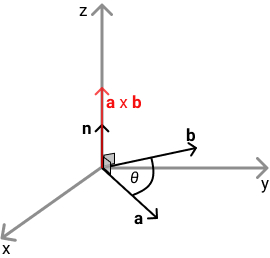
\includegraphics[scale=0.5]{img/cross-product-1.jpg}
\end{figure}

Una primera caracteristica del producto cruz $\mathbf{a} \times \mathbf{b}$, es que corresponde a \textbf{un vector}. Más específicamente, es $\mathbf{n}$ escalado por el factor $(||\mathbf{a}|| \cdot ||\mathbf{b}|| \cdot \sin(\theta))$, lo que implica que:
\[
  (\mathbf{a} \times \mathbf{b}) \perp \mathbf{a} \qquad \text{y} \qquad (\mathbf{a} \times \mathbf{b}) \perp \mathbf{b}
\]
Otra particularidad de $\mathbf{a} \times \mathbf{b}$, es que \textbf{solo se aplica en el espacio}. Es decir, podemos calcular el producto cruz entre dos vectores siempre que \textbf{ambos estén en tres dimensiones}.

Una tercera característica del producto cruz, es que será igual al vector $\mathbf{0}$ si $\mathbf{a}$ y $\mathbf{b}$ son \textbf{paralelos}. Geométricamente, significa que $\theta = 0$ o $\theta = \pi$. Por lo tanto:
\begin{align*}
\mathbf{a} \times \mathbf{b} &= (||\mathbf{a}|| \cdot ||\mathbf{b}|| \cdot \sin(0)) \cdot \mathbf{n} = \mathbf{0} &
\mathbf{a} \times \mathbf{b} &= (||\mathbf{a}|| \cdot ||\mathbf{b}|| \cdot \sin(\pi)) \cdot \mathbf{n} = \mathbf{0}
\end{align*}
También $\mathbf{a}$ y $\mathbf{b}$ serán paralelos si \textbf{son iguales}.
\[
  \mathbf{a} \times \mathbf{b} = \mathbf{0} \iff \mathbf{a} = \mathbf{b}
\]

\subsection{Magnitud y Dirección del Producto Cruz.}

La \textbf{magnitud} de $\mathbf{a} \times \mathbf{b}$ coincide con ser el \textbf{área de un paralelógramo en el espacio}. Recordemos que es el producto escalar $(||\mathbf{a}|| \cdot ||\mathbf{b}|| \cdot \sin(\theta)) \cdot \mathbf{n}$, por lo tanto:
\[
  ||\mathbf{a} \times \mathbf{b}|| = (||\mathbf{a}|| \cdot ||\mathbf{b}|| \cdot \sin(\theta)) \cdot ||\mathbf{n}||
\]
Como $\mathbf{n}$ es un vector unitario (i.e, $||\mathbf{n}|| = 1$), entonces:

\[
  ||\mathbf{a} \times \mathbf{b}|| = ||\mathbf{a}|| \cdot ||\mathbf{b}|| \cdot \sin(\theta)
\]
En la sección anterior (pág. 4), vimos que el lado derecho de la expresión de arriba corresponde al área de un paralelógramo generado por dos vectores no nulos $\mathbf{a}$ y $\mathbf{b}$. Es decir:
\[
  ||\mathbf{a} \times \mathbf{b}|| = A_{P}
\]

\begin{figure}[hbt!]
\centering
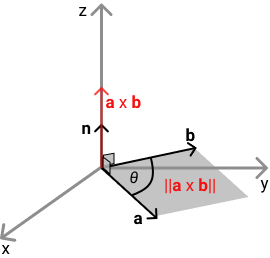
\includegraphics[scale=0.6]{img/cross-product-2.jpg}
\end{figure}

Para conocer la \textbf{dirección del producto cruz}, usamos la \textbf{regla de la mano derecha}, que consiste en mantenerla abierta de forma opuesta al arco del ángulo, para después cerrarla. La dirección de este vector será el \textbf{lugar a donde apunte nuestro dedo pulgar}.

\begin{figure}[hbt!]
\centering
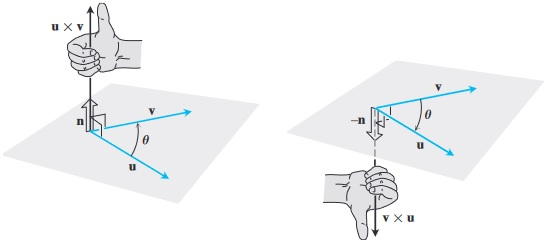
\includegraphics[scale=0.75]{img/right-hand-rule.jpg}
\caption{Thomas (2010). \textit{Cálculo. Varias Variables}. Pp. 682-683.}
\end{figure}

\subsection{Propiedades del Producto Cruz.}

Sean $\mathbf{a}$, $\mathbf{b}$ y $\mathbf{w}$ tres vectores cualquiera y $c$ y $d$ escalares, el producto cruz cumple con las siguiente propiedades:
\begin{align*}
&1) \ (c\mathbf{a}) \times (d\mathbf{b}) = (cd) (\mathbf{a} \times \mathbf{b}) &
&2) \ \mathbf{a} \times (\mathbf{b} + \mathbf{w}) = \mathbf{a} \times \mathbf{b} + \mathbf{a} \times \mathbf{w} \\
&3) \ \mathbf{a} \times \mathbf{b} = -(\mathbf{b} \times \mathbf{a}) &
&4) \ (\mathbf{a} + \mathbf{b}) \times \mathbf{w} = \mathbf{a} \times \mathbf{w} + \mathbf{b} \times \mathbf{w} \\
&5) \ \mathbf{0} \times \mathbf{a} = \mathbf{0} &
&6) \ \mathbf{a} \times (\mathbf{b} \times \mathbf{w}) = (\mathbf{a} \cdot \mathbf{w})\mathbf{b} - (\mathbf{a} \cdot \mathbf{b}) \mathbf{w}
\end{align*}

Ahora, sean los vectores unitarios estándar $\hat{\mathbf{i}} = \langle 1, \ 0, \ 0 \rangle$, $\hat{\mathbf{j}} = \langle 0, \ 1, \ 0 \rangle$ y $\hat{\mathbf{k}} = \langle 0, \ 0, \ 1 \rangle$. Aplicando la propiedad 3) vista anteriormente, podemos obtener las siguientes igualdades:
\begin{align*}
  \hat{\mathbf{i}} \times \hat{\mathbf{j}} &= -(\hat{\mathbf{j}} \times \hat{\mathbf{i}}) = \hat{\mathbf{k}} \\
  \hat{\mathbf{j}} \times \hat{\mathbf{k}} &= -(\hat{\mathbf{k}} \times \hat{\mathbf{j}}) = \hat{\mathbf{i}} \\
  \hat{\mathbf{k}} \times \hat{\mathbf{i}} &= -(\hat{\mathbf{i}} \times \hat{\mathbf{k}}) = \hat{\mathbf{j}}
\end{align*}
También podemos asegurar que:
\[
  \hat{\mathbf{i}} \times \hat{\mathbf{i}} = \hat{\mathbf{j}} \times \hat{\mathbf{j}} = \hat{\mathbf{k}} \times \hat{\mathbf{k}} = \mathbf{0}
\]
Estas igualdades con los tres vectores unitarios podemos observarlas a continuación:

\begin{figure}[hbt!]
\centering
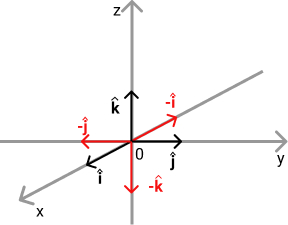
\includegraphics[scale=0.6]{img/cross-product-3.jpg}
\end{figure}

\subsection{Producto Cruz a partir de los componentes.}

Hasta ahora sabemos calcular el producto cruz entre dos vectores considerando el ángulo que se forma entre ellos. A partir de las propiedades estudiadas en la subsección anterior, podemos obtener a este vector solo con los componentes de ambos.

Suponga que $\mathbf{a} = a_{1} \hat{\mathbf{i}} + a_{2} \hat{\mathbf{j}} + a_{3} \hat{\mathbf{k}}$ y $\mathbf{b} = b_{1} \hat{\mathbf{i}} + b_{2} \hat{\mathbf{j}} + b_{3} \hat{\mathbf{k}}$. Entonces:
\begin{align*}
\mathbf{a} \times \mathbf{b} = &(a_{1} \hat{\mathbf{i}} + a_{2} \hat{\mathbf{j}} + a_{3} \hat{\mathbf{k}}) \times
                                (b_{1} \hat{\mathbf{i}} + b_{2} \hat{\mathbf{j}} + b_{3} \hat{\mathbf{k}}) \\
                             = &(a_{1} \hat{\mathbf{i}} + a_{2} \hat{\mathbf{j}} + a_{3} \hat{\mathbf{k}}) \times b_{1} \hat{\mathbf{i}} + 
                                (a_{1} \hat{\mathbf{i}} + a_{2} \hat{\mathbf{j}} + a_{3} \hat{\mathbf{k}}) \times b_{2} \hat{\mathbf{j}} + 
                               (a_{1} \hat{\mathbf{i}} + a_{2} \hat{\mathbf{j}} + a_{3} \hat{\mathbf{k}}) \times b_{3} \hat{\mathbf{k}} \\
\mathbf{a} \times \mathbf{b} = &a_{1}b_{1}(\hat{\mathbf{i}} \times \hat{\mathbf{i}}) + a_{2}b_{1}(\hat{\mathbf{j}} \times \hat{\mathbf{i}}) +
                               a_{3}b_{1}(\hat{\mathbf{k}} \times \hat{\mathbf{i}}) + a_{1}b_{2}(\hat{\mathbf{i}} \times \hat{\mathbf{j}}) +
                               a_{2}b_{2}(\hat{\mathbf{j}} \times \hat{\mathbf{j}}) + a_{3}b_{2}(\hat{\mathbf{k}} \times \hat{\mathbf{j}}) + \\
                               &a_{1}b_{3}(\hat{\mathbf{i}} \times \hat{\mathbf{k}}) + a_{2}b_{3}(\hat{\mathbf{j}} \times \hat{\mathbf{k}}) +
                                a_{3}b_{3}(\hat{\mathbf{k}} \times \hat{\mathbf{k}})
\end{align*}
Apliquemos las igualdades de los vectores unitarios vistas en las propiedades del producto cruz en la ecuación de arriba y reordenémosla.
\begin{align*}
\mathbf{a} \times \mathbf{b} = &(a_{1}b_{1}) \mathbf{0} + (a_{2}b_{2}) \mathbf{0} + (a_{3}b_{3}) \mathbf{0} + \\
                               &(a_{2}b_{3})\hat{\mathbf{i}} - (a_{3}b_{2}) \hat{\mathbf{i}} - (a_{1}b_{3}) \hat{\mathbf{j}} +
                                (a_{3}b_{1}) \hat{\mathbf{j}} + (a_{1}b_{2}) \hat{\mathbf{k}} - (a_{2}b_{1}) \hat{\mathbf{k}} \\
\mathbf{a} \times \mathbf{b} = &(a_{2}b_{3} - a_{3}b_{2}) \hat{\mathbf{i}} - (a_{1}b_{3} - a_{3}b_{1}) \hat{\mathbf{j}} +
                                (a_{1}b_{2} - a_{2}b_{1}) \hat{\mathbf{k}}
\end{align*}
Por lo tanto, el producto cruz entre $\mathbf{a}$ y $\mathbf{b}$ calculado a partir de sus componentes se obtiene como:
\[
\mathbf{a} \times \mathbf{b} = (a_{2}b_{3} - a_{3}b_{2}) \hat{\mathbf{i}} - (a_{1}b_{3} - a_{3}b_{1}) \hat{\mathbf{j}} + 
                               (a_{1}b_{2} - a_{2}b_{1}) \hat{\mathbf{k}}
\]
Veamos una forma más sencilla de recordar esta fórmula. Si observamos bien, la ecuación del producto cruz es similar en su forma a la del \textbf{determinante en el espacio}, salvo que tenemos vectores en ella. Por lo tanto, es posible escribirla \textbf{simbólicamente} como:
\[
\mathbf{a} \times \mathbf{b} =
\begin{vmatrix}
\hat{\mathbf{i}} & \hat{\mathbf{j}} & \hat{\mathbf{k}} \\
a_{1} & a_{2} & a_{3} \\
b_{1} & b_{2} & b_{3}
\end{vmatrix} =
\hat{\mathbf{i}} \cdot
\begin{vmatrix}
a_{2} & a_{3} \\
b_{2} & b_{3}
\end{vmatrix}
- \hat{\mathbf{j}} \cdot
\begin{vmatrix}
a_{1} & a_{3} \\
b_{1} & b_{3}
\end{vmatrix}
+ \hat{\mathbf{k}} \cdot
\begin{vmatrix}
a_{1} & a_{2} \\
b_{1} & b_{2}
\end{vmatrix}
\]
Ojo que solo escribimos el producto cruz como un determinante de forma simbólica, ya que éste último, en realidad, nos entrega un valor escalar y no vectorial, pero es útil para recordar más fácilmente su fórmula.

\subsection{El Triple Producto Escalar.}

Antes de terminar, volvamos a estudiar el volumen de un paralelepipedo $V_{P}$ generado por $\mathbf{a}$, $\mathbf{b}$ y $\mathbf{c}$.

\newpage

\begin{figure}[hbt!]
\centering
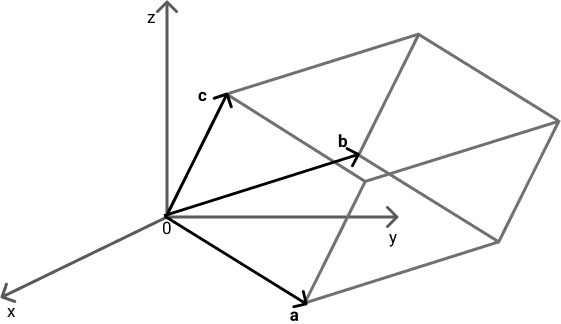
\includegraphics[scale=0.4]{img/det-vol-parallelel-1.jpg}
\end{figure}

Demostremos que:
\[
  V_{P} = |\det(\mathbf{a}, \ \mathbf{b}, \ \mathbf{c})|
\]
\textbf{Demostración}. En términos generales, el volumen de un sólido como el paralelepipedo se calcula de la siguiente manera:
\[
V_{P} = A(\text{base}) \cdot h
\]
donde $A(\text{base})$ es el área de su base y $h$ su altura.

La base de este paralelepipedo es un paralelógramo, el cual coincide con estar formado por los vectores $\mathbf{a}$ y $\mathbf{b}$. Por lo tanto, su área podemos calcularla como la magnitud del producto cruz entre ambos.
\[
  A(\text{base}) = ||\mathbf{a} \times \mathbf{b}||
\]
En cuanto a la altura del paralelepipedo, como es perpendicular a su base, podemos obtenerla como el componente $c_{3}$ de $\mathbf{c}$ en dirección de un vector $\mathbf{n}$ unitario y ortogonal a dicho plano.

\begin{figure}[hbt!]
\centering
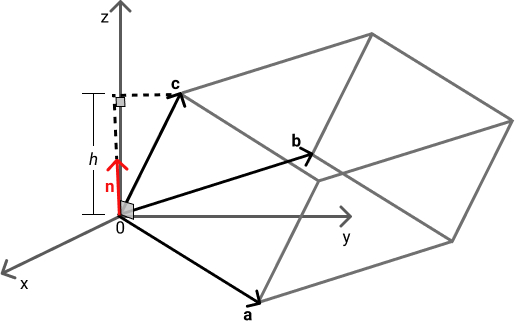
\includegraphics[scale=0.4]{img/triple-product-1.jpg}
\end{figure}

Es decir:
\[
  h = \mathbf{c} \cdot \mathbf{n}
\]
Como el vector unitario $\mathbf{n}$ es perpendicular a la base del paralelepipedo, entonces es equivalente al $\mathbf{a} \times \mathbf{b}$ normalizado, porque al ser ortogonal a $\mathbf{a}$ y a $\mathbf{b}$, también lo es a aquella superficie.
\[
  h = \mathbf{c} \cdot \frac{\mathbf{a} \times \mathbf{b}}{||\mathbf{a} \times \mathbf{b}||}, \quad \text{donde }
  \mathbf{n} = \left(\frac{\mathbf{a} \times \mathbf{b}}{||\mathbf{a} \times \mathbf{b}||}\right)
\]
Por lo tanto:
\[
  V_{P} = ||\mathbf{a} \times \mathbf{b}|| \cdot
          \left(\mathbf{c} \cdot \frac{\mathbf{a} \times \mathbf{b}}{||\mathbf{a} \times \mathbf{b}||}\right)
        = \mathbf{c} \cdot (\mathbf{a} \times \mathbf{b})
\]
La operación $\mathbf{c} \cdot (\mathbf{a} \times \mathbf{b})$ se conoce como \textbf{Triple Producto Escalar}, puesto que es el producto punto entre el vector de la izquierda y el producto cruz de la derecha.

Para calcular un triple producto escalar, siempre comenzamos con el producto cruz y después con el producto punto.

Entonces, sean $\mathbf{c} = \langle c_{1}, \ c_{2}, \ c_{3} \rangle$ y $\mathbf{a} \times \mathbf{b} = \langle (a_{2}b_{3} - a_{3}b_{2}), \ (a_{3}b_{1} - a_{1}b_{3}), \ (a_{1}b_{2} - a_{2}b_{1}) \rangle$, el volumen del paralelepipedo $V_{P}$ corresponde a:
\begin{align*}
V_{P} &= \mathbf{c} \cdot (\mathbf{a} \times \mathbf{b}) \\
      &= c_{1}(a_{2}b_{3} - a_{3}b_{2}) + c_{2}(a_{3}b_{1} - a_{1}b_{3}) + c_{3}(a_{1}b_{2} - a_{2}b_{1}) \\
      &= a_{2}b_{3}c_{1} - a_{3}b_{2}c_{1} + a_{3}b_{1}c_{2} - a_{1}b_{3}c_{2} + a_{1}b_{2}c_{3} - a_{2}b_{1}c_{3} \\
      &= a_{1}(b_{2}c_{3}- b_{3}c_{2}) - a_{2}(b_{1}c_{3} - b_{3}c_{1}) + a_{3}(b_{1}c_{2} - b_{2}c_{1}) \\
      &= a_{1} \cdot
         \begin{vmatrix}
         b_{2} & b_{3} \\
         c_{2} & c_{3}
         \end{vmatrix}
         - a_{2} \cdot
         \begin{vmatrix}
         b_{1} & b_{3} \\
         c_{1} & c_{3}
         \end{vmatrix}
         + a_{3} \cdot
         \begin{vmatrix}
         b_{1} & b_{2} \\
         c_{1} & c_{2}
         \end{vmatrix} \\
      &= \begin{vmatrix}
         a_{1} & a_{2} & a_{3} \\
         b_{1} & b_{2} & b_{3} \\
         c_{1} & c_{2} & c_{3}
         \end{vmatrix} \\
V_{P} &= |\det(\mathbf{a}, \ \mathbf{b}, \ \mathbf{c})| \quad (\text{Q. E. D})
\end{align*}
El volumen del paralelepipedo podemos interpretarlo como el determinante entre $\mathbf{a}$, $\mathbf{b}$ y $\mathbf{c}$ en el espacio, el cual es igual al triple producto entre $\mathbf{c}$ y el producto cruz $\mathbf{a} \times \mathbf{b}$.


\end{document}
